\counterwithin{figure}{section}
\section{Problem Definition}
In the project, it is required to drive a DC motor with AC voltage from variac. Motor will be connected to a DC generator that will be connected to a kettle which will boil water so that we can drink tea.

DC motor can be observed in the Figure \ref{motor-set} below:

\begin{center}
\begin{figure}[H]
\centering
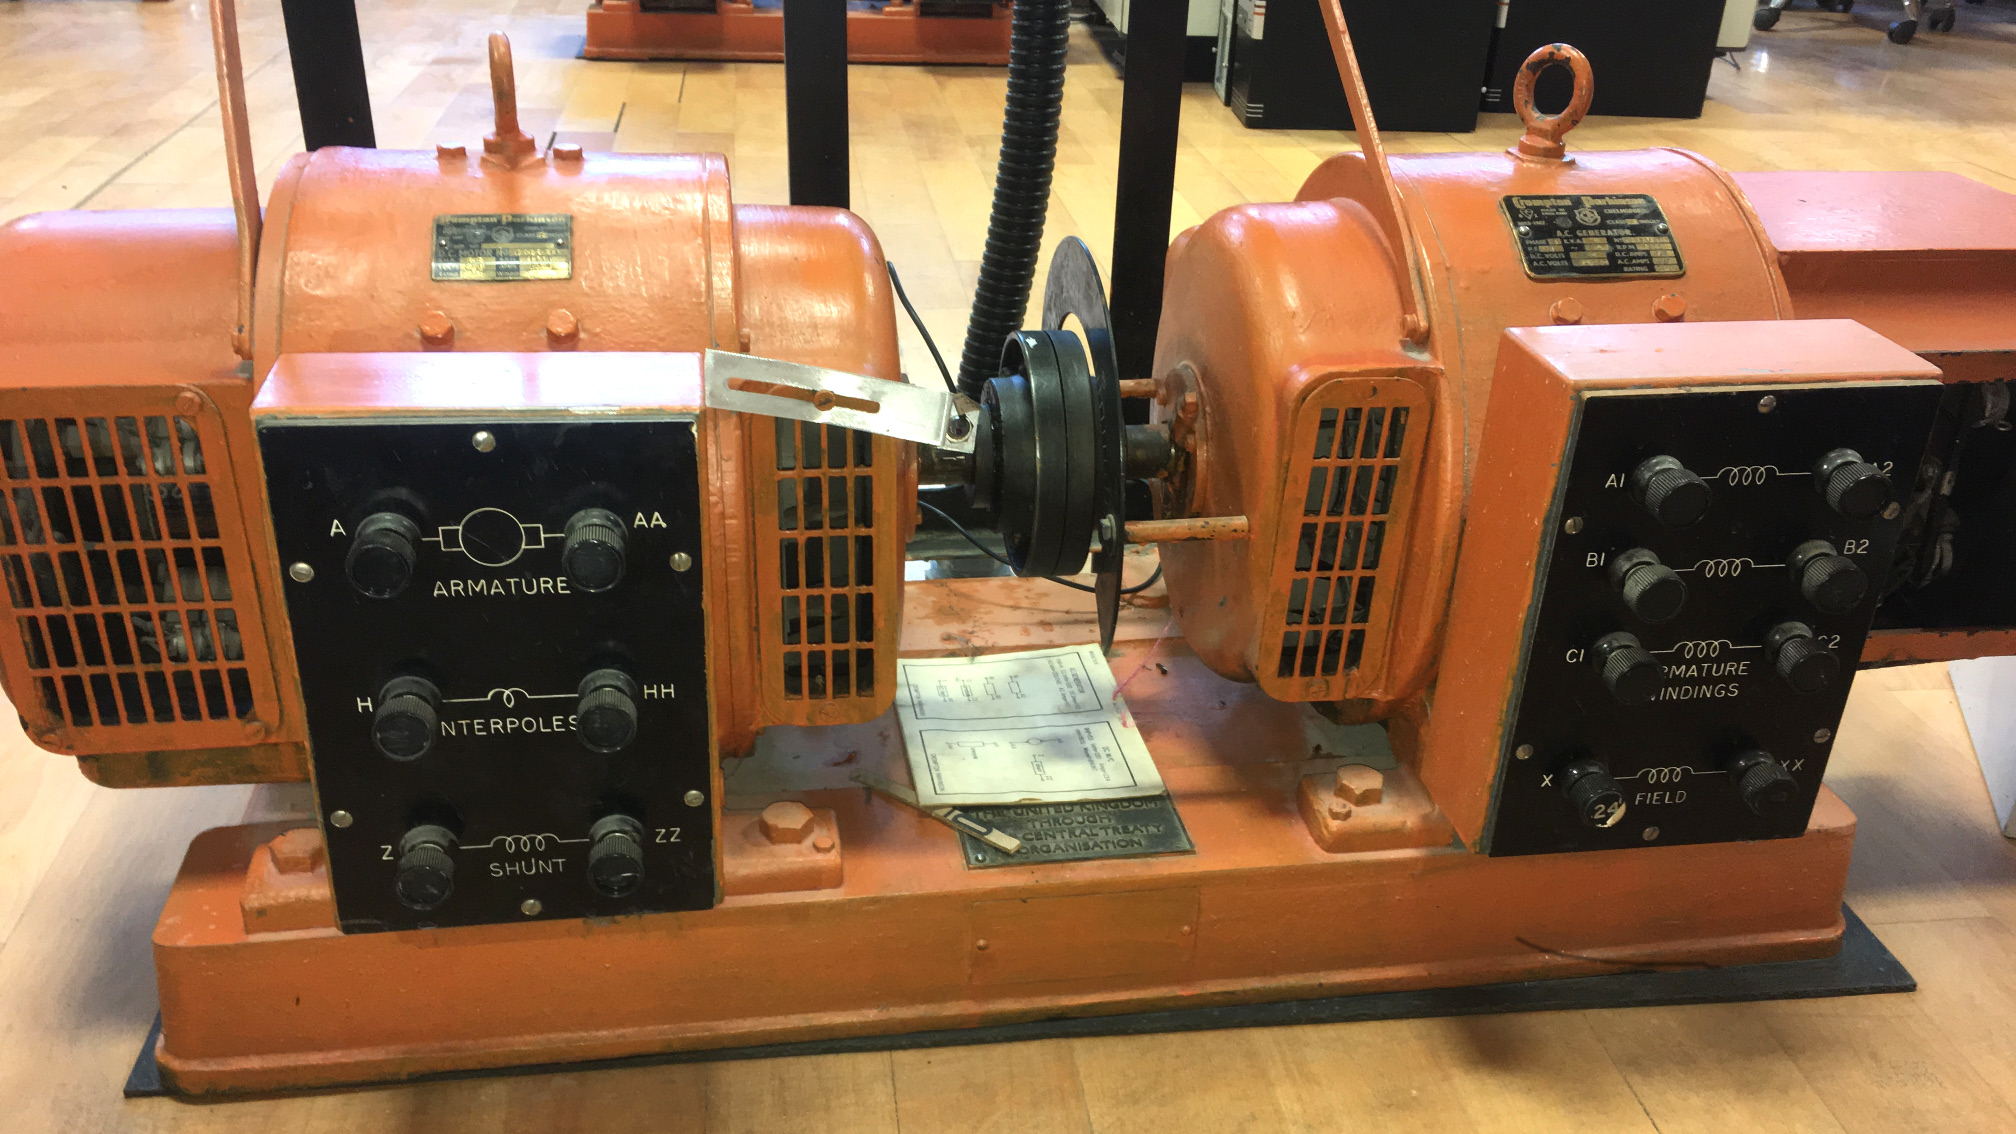
\includegraphics [width= 12 cm ]{motor-set}
\caption{DC Motor}
\label{motor-set}
\end{figure}
\end{center}

Parameters of the DC Motor:
\begin{itemize}
    \item Armature Winding: 0.8 \ohm, 12.5 mH
    \item Shunt Winding: 210 \ohm, 23 H
    \item Interpoles Winding: 0.27 \ohm, 12 mH
\end{itemize}

Requirements are:
\begin{itemize}
    \item Input is single-phase or three-phase AC Voltage
    \item Output, $V_{dc,max} < 180 V$
\end{itemize}
